\section{The Onset of Vocabulary Acceleration}
\label{sec:vocab_accel}
Our previous experiments confirm that simple neural networks can develop the shape
bias when presented with realistic human training sets. It remains unclear,
however, how this bias influences word learning. \cite{GershkoffStowe2004}
showed that the development of the shape bias in infants is correlated with the
onset of vocabulary accceleration; children who displayed a stronger shape bias
in the study exhibited a higher rate of vocabulary acquisition. Eight children subjects
participated in the study, beginning at ages 16 to 20 months. The vocabulary
of each subject was monitored over the course of the study. Every three weeks,
the shape bias level of each subject was evaluated in the lab using a test
akin to the second-order generalization test of \cite{Smith2002}. Authors of the
study reported a number of interesting findings regarding the relationship between
generalization performance and the number of nouns in a child's vocabulary. First,
they found a correlation of 0.7 between generalization performance and the rate of
change in the number of nouns possessed over the course of the study. TODO:
discuss other findings of the study.

\begin{figure}[t!]
    \begin{center}
        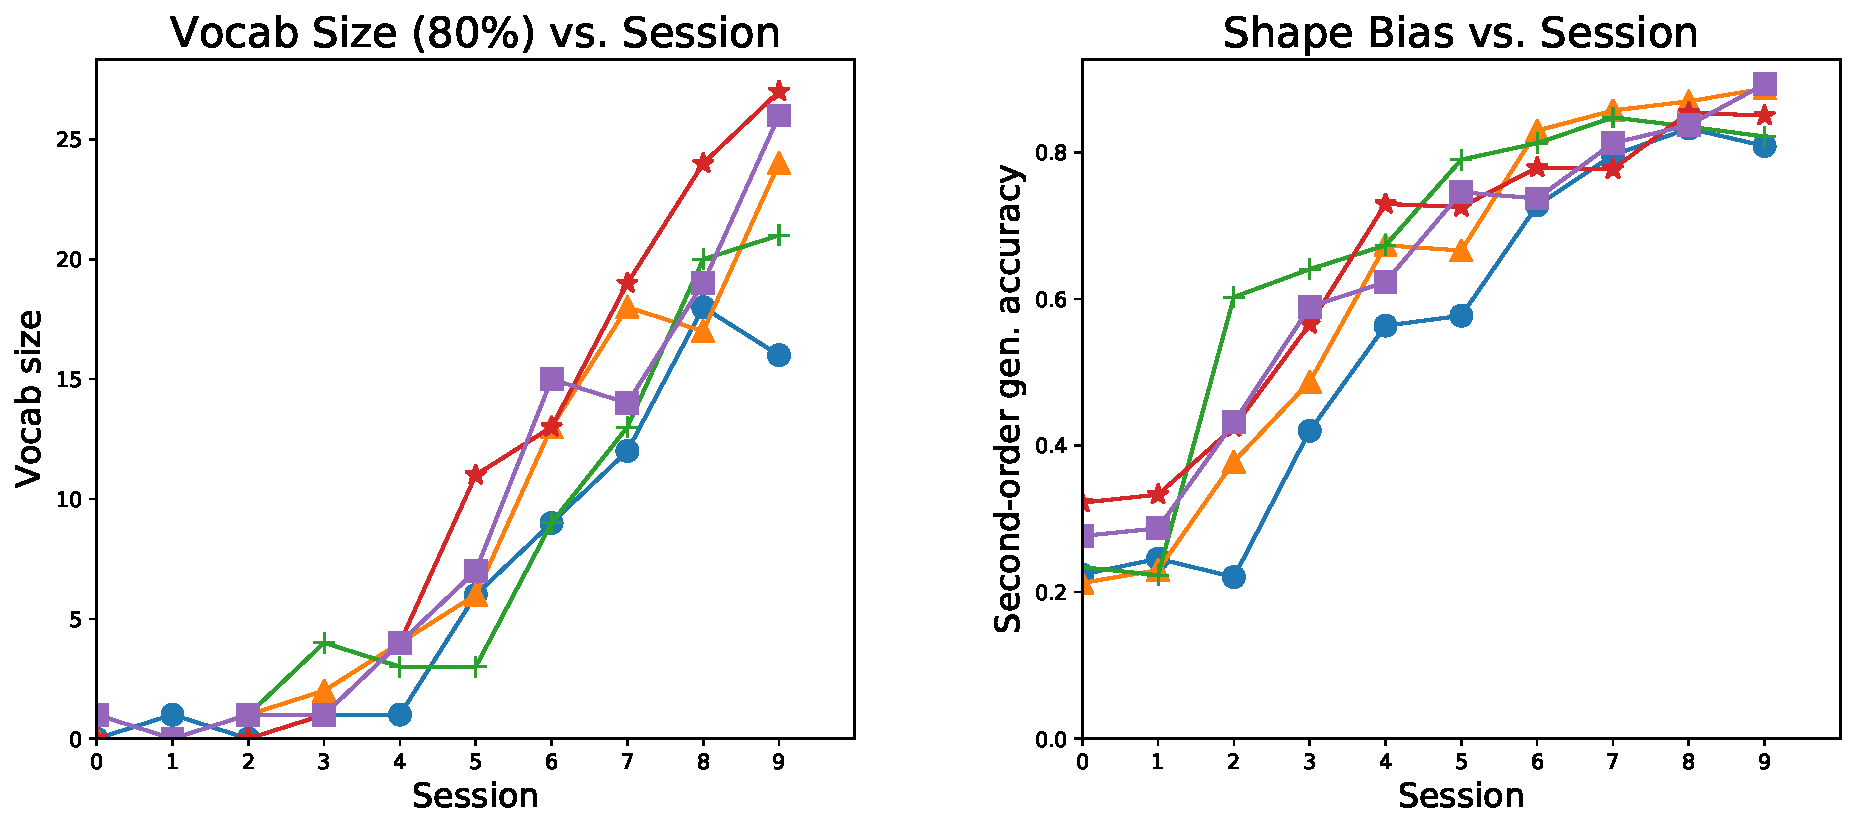
\includegraphics[width=0.49\textwidth]{figures/shapebias_and_vocab.pdf}
    \end{center}
    \caption{Learning curves for shape bias and vocabulary size of a CNN. TODO:
    update these plots, update caption.}
    \label{fig:learning_curves}
\end{figure}

We replicated this experiment to the best of our ability using a CNN and our
RGB image data. We trained a series of eight networks using 50 categories and
20 exemplars of each category. Fig. \ref{fig:learning_curves} shows plots that
miror Figures 5 \& 6 of \cite{GershkoffStowe2004}. TODO: update this explaination.
TODO: finish vocabulary acceleration experiments.